\section{Load Calculations}
\label{app:loadcalc}
\setcounter{equation}{0}
At EML2, the gravitational acceleration is nearly zero, the force acting on the arm is coming from external contact like EVA or the acceleration of payload.

\large \textbf{Payload reaction force/torque}\\
\normalsize There is no moving speed and stopping distance requirement proposed by customer. However, we can use the performance of reference design such as Canadarm and Canadarm2 to calculate a reference loading requirement. 

Tip velocity of Canadarm with full payload:$v=0.06m/s$\\
Canadarm stopping distance with full payload: $b=0.6m$\\
Leaving a 30\% margin, Stopping Distance: $b=0.42m$\\
Maximum payload mass from RFP: $m=10000kg$

Assume payload acceleration is constant, the following two equations are used to calculate acceleration:
\begin{equation}
b=v_it+\frac{1}{2}at^2
\end{equation}
\begin{equation}
a=\frac{v_f-v_i}{t}
\end{equation}
where:\\
$v_i=v$ is the initial velocity of payload\\
$v_f=0$ is the final velocity of payload\\
This gives us a result of $$t=14s, a=0.0043m/s^2$$

The reaction force applied by the payload is 
$$F=ma=10000kg\times0.0043m/s^2=43N$$

This reaction force will apply a bending moment to the robotic arm. Another type of load applied by the payload is torque due to the rotational motion. Canadarm2's rotational velocity and stopping angle are used. 

Rotational Velocity: $\omega=0.24\deg/s=0.0042rad/s$ \cite{NASAsysreq_Kumar}\\
Rotational Stopping Distance: $\theta=3.8\deg$
Leaving a 30\% margin, Stopping Distance: $\theta=2.9\deg=0.051rad$

These two performance characteristics of Canadarm2 are associated with payload that has mass of \SI{209000}{\kilo\gram} and size of \SI{4.5}{\metre} in diameter and \SI{17}{\metre} in length. This mass is twice of the maximum required in RFP and the size of the payload was not specified in the RFP. The size of the payload handled by the robotic system is assumed half the length of Canadarm2 payload. This size is also a close resemblance of a service module on ISS \cite{ISS_Harmony}.

Maximum payload mass from RFP: $m=10000kg$
Payload size: diameter $d=4.5 m$; length $l=8.5 m$
Assume payload has uniform density, payload moment of inertia:
$$I=\frac{1}{4}m(\frac{d}{2})^2+\frac{1}{2}ml^2=253490 kg\cdot m^2$$
The axis for the moment of inertia is chosen according to the location of the grapple fixture on the ISS module\cite{ISS_Harmony}. The axis is marked as a black dotted line in \Cref{fig:harmony_axis}.

\begin{figure}[H]
\centering
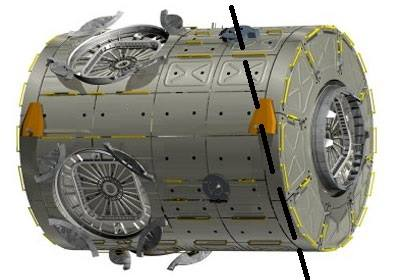
\includegraphics[width=0.4\textwidth]{Apppic/harmony}
\caption{Axis used to calculate moment of inertia}
\label{fig:harmony_axis}
\end{figure}

Assuming payload rotational acceleration is constant, the following two equations are used to calculate rotational acceleration.
\begin{equation}
\theta=\omega_it+\frac{1}{2}\alpha t^2
\end{equation}
\begin{equation}
\alpha=\frac{(\omega_f-\omega_i)}{t}
\end{equation}
where:\\
$\omega_i=\omega$ is the initial rotational velocity of payload\\
$\omega_f=0$ is the final rotational velocity of payload

This gives us the result of $$t=24s, \alpha=0.00177rad/s^2$$
The reaction torque applied by the payload is then
$$\tau=I\alpha=253490kg\cdot m^2\times 0.00177rad/s^2=448.7Nm$$

\large \textbf{Holding/Reaction forces}\\
\normalsize Requirement \textbf{EE-P-02} states that the end effector subsystem shall apply holding or reaction forces of \SI{200}{\newton} in any direction.

\large \textbf{Holding/Reaction forces}\\
\normalsize The robotic arm can be modeled as a cantilever beam and the highest load occurs when the arm is straight as shown in \Cref{fig:loading} below. The holding and reaction force is higher than the payload reaction force, therefore the force of \SI{200}{\newton} from holding and reaction is used.

\begin{figure}[H]
\centering
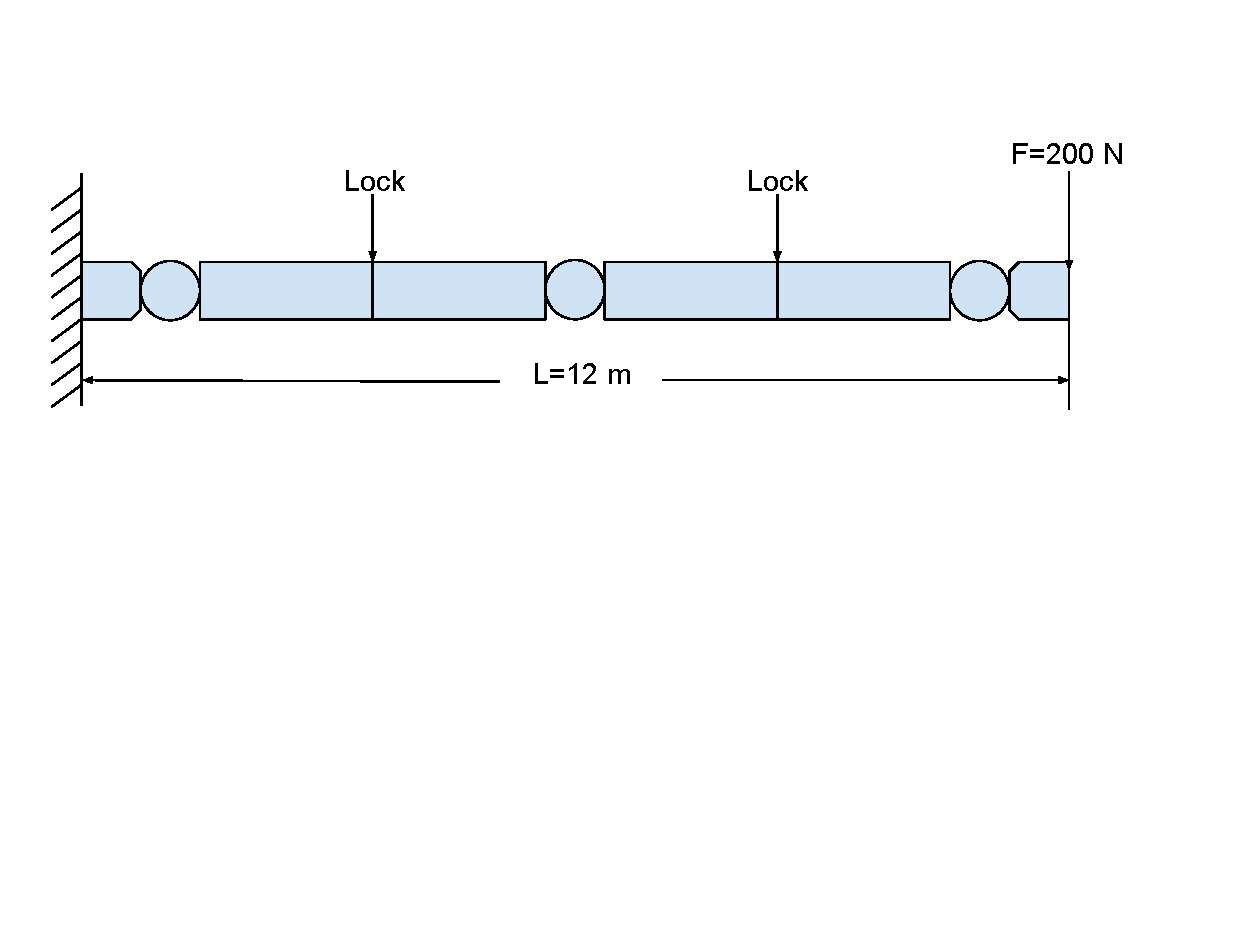
\includegraphics[width=0.6\textwidth]{Apppic/loading}
\caption{Maximum loading configuration of system}
\label{fig:loading}
\end{figure}

The maximum moment is at the end effector and shoulder joint.
$$M=FL=2400Nm$$
The moment at the lock where the telescopic boom is locked is:
$$M_{Lock} = FL_{Lock} = 1800 Nm$$
The moment at the elbow joint is:
$$M_{elbow} = FL_{elbow} = 1200 Nm$$
Given factor of safety of 1.5, the final bending moments on the arm are:
$$M =3600 Nm, M_{Lock} =2700 Nm, M_{elbow} =1800 Nm$$
The rotational torque load on the arm is:
$$T = 448.7 Nm\cdot1.5=673.05 Nm$$

\large \textbf{Other reference load requirement}\\
\normalsize \textbf{End Effector}\\
The end effectors of Canadarm2 need to perform snare, rigidize and latch mechanism, the load transfer capability of the end effector are \cite{NASAsysreq_Kumar}:\\
i) ``\SI{950}{\newton\metre} torque and \SI{1220}{\newton\metre} bending moment when snared and rigidized, allowing \SI{3}{\degree} separation at the interface."\\
ii) ``\SI{3210}{\newton\metre} moment about any axis and \SI{1110}{\newton\metre} axial/shear force when snared, rigidized and latched and no separation at the interface"

\textbf{Vibrational Load}\\
During the launch of the aircraft, the robotic system will experience vibrational load and shock load due to engine firing and engine cut off. While the type of the launch vehicle is specified in RFP, the common launch vehicles used are Atlas V and Delta IV, and design characteristics use these vehicles. The vibration design, shock design and testing characteristics are presented in \Cref{delta_launch,atlas_launch} below

\begin{table}[H]
\centering
\caption[Vibration design, shock design and testing characteristics of Delta IV]{Vibration design, shock design and testing characteristics of Delta IV \cite{delta_launch}}
\begin{tabular}{|c|c|c|c|}
\hline
	&	\textbf{Frequency (Hz)}	&	\textbf{Test Level}	&	\textbf{Sweep Rate}	\\\hhline{|=|=|=|=|}
{\textbf{Sinusoidal Vibration}}	&	5 to 7.4	&	\SI{1.27}{\centi\metre}double amplitude	&	\multirow{2}{*}{2 octaves/min}	\\\cline{2-3}
{\textbf{Axial}}	&	7.4 to 100	&	1.4g (zero to peak)	&	\\\hline
{\textbf{Sinusoidal Vibration}}	&	5 to 6.2	&	\SI{1.27}{\centi\metre}double amplitude	&	\multirow{2}{*}{2 octaves/min}	\\\cline{2-3}
{\textbf{Lateral}}	&	6.2 to 100	&	1.0g (zero to peak)	&	\\\hline
\textbf{Shock}	&	150	&	120g	&	N/A	\\\hline

\end{tabular}
\label{delta_launch}
\end{table}

\begin{table}[H]
\centering
\caption[Vibration design, shock design and testing characteristics of Atlas V]{Vibration design, shock design and testing characteristics of Atlas V \cite{atlas_launch}}
\begin{tabular}{|c|c|c|c|}
\hline
	&	\textbf{Frequency (Hz)}	&	\textbf{Test Level}	&	\textbf{Sweep Rate}	\\\hhline{|=|=|=|=|}
{\textbf{Sinusoidal Vibration}}	&	\multirow{2}{*}{5 to 100}	&	\multirow{2}{*}{1.125g (zero to peak)}	&	\multirow{2}{*}{2 octaves/min}	\\
{\textbf{Axial}}	&		&		&	\\\hline
{\textbf{Sinusoidal Vibration}}	&	\multirow{2}{*}{5 to 100}	&	\multirow{2}{*}{0.75g (zero to peak)}	&	\multirow{2}{*}{2 octaves/min}	\\
{\textbf{Axial}}	&		&		&	\\\hline
\textbf{Shock}	&	270	&	120g	&	N/A	\\\hline
\end{tabular}
\label{atlas_launch}
\end{table}



